\chapter{Задача о назначениях}
Решить задачу о назначениях с помощью венгерского алгоритма.\\
Имеется n видов ресурсов, которые нужно распределить на n объектов, n = 10.\\
$c_{ij}$ - затраты, связанные с назначением i-го ресурса на j-й объект.\\
Каждый ресурс назначается ровно один раз и каждому объекту приписывается ровно один ресурс.\\
Требуется минимизировать стоимость назначений.

\begin{center}
    \begin{tabular}{|a | c | c | c | c | c | c | c | c | c | c|} 
         \hline
         \rowcolor{LightGray}
            & 1 & 2 & 3 & 4 & 5 & 6 & 7 & 8 & 9 & 10\\
         \hline
            1 & 1 & 3 & 6 & 4 & 7 & 1 & 8 & 2 & 8 & 3\\
         \hline
            2 & 1 & 6 & 4 & 9 & 8 & 3 & 5 & 7 & 1 & 2\\
         \hline
            3 & 8 & 1 & 5 & 9 & 3 & 6 & 4 & 7 & 7 & 9\\
         \hline
            4 & 3 & 6 & 1 & 9 & 2 & 4 & 5 & 8 & 3 & 5\\
        \hline
            5 & 2 & 7 & 9 & 4 & 1 & 2 & 8 & 9 & 5 & 2\\
         \hline
            6 & 7 & 1 & 8 & 6 & 3 & 2 & 4 & 7 & 9 & 5\\
         \hline
            7 & 6 & 8 & 5 & 9 & 2 & 4 & 7 & 1 & 2 & 3\\
         \hline
            8 & 2 & 4 & 7 & 5 & 9 & 1 & 4 & 8 & 7 & 3\\
        \hline
            9 & 7 & 1 & 6 & 9 & 3 & 2 & 5 & 3 & 4 & 2\\
         \hline
            10 & 6 & 4 & 7 & 5 & 9 & 4 & 5 & 8 & 1 & 3\\
        \hline
    \end{tabular}
\end{center}

\begin{center}
    {\bf
    Решение:}
\end{center}

\begin{center}
    \begin{tabular}{|a | c | c | c | c | c | c | c | c | c | c | g|} 
         \hline
         \rowcolor{LightGray}
            & 1 & 2 & 3 & 4 & 5 & 6 & 7 & 8 & 9 & 10 & min\\
         \hline
            1 & 1 & 3 & 6 & 4 & 7 & 1 & 8 & 2 & 8 & 3 & 1\\
         \hline
            2 & 1 & 6 & 4 & 9 & 8 & 3 & 5 & 7 & 1 & 2 & 1\\
         \hline
            3 & 8 & 1 & 5 & 9 & 3 & 6 & 4 & 7 & 7 & 9 & 1\\
         \hline
            4 & 3 & 6 & 1 & 9 & 2 & 4 & 5 & 8 & 3 & 5 & 1\\
        \hline
            5 & 2 & 7 & 9 & 4 & 1 & 2 & 8 & 9 & 5 & 2 & 1\\
         \hline
            6 & 7 & 1 & 8 & 6 & 3 & 2 & 4 & 7 & 9 & 5 & 1\\
         \hline
            7 & 6 & 8 & 5 & 9 & 2 & 4 & 7 & 1 & 2 & 3 & 1\\
         \hline
            8 & 2 & 4 & 7 & 5 & 9 & 1 & 4 & 8 & 7 & 3 & 1\\
        \hline
            9 & 7 & 1 & 6 & 9 & 3 & 2 & 5 & 3 & 4 & 2 & 1\\
         \hline
            10 & 6 & 4 & 7 & 5 & 9 & 4 & 5 & 8 & 1 & 3 & 1\\
        \hline
    \end{tabular}
\end{center}

\begin{center}
    \begin{tabular}{|a | c | c | c | c | c | c | c | c | c | c|} 
         \hline
         \rowcolor{LightGray}
            & 1 & 2 & 3 & 4 & 5 & 6 & 7 & 8 & 9 & 10\\
         \hline
            1 & 0 & 2 & 5 & 3 & 6 & 0 & 7 & 1 & 7 & 2\\
         \hline
            2 & 0 & 5 & 3 & 8 & 7 & 2 & 4 & 6 & 0 & 1\\
         \hline
            3 & 7 & 0 & 4 & 8 & 2 & 5 & 3 & 6 & 6 & 8\\
         \hline
            4 & 2 & 5 & 0 & 8 & 1 & 3 & 4 & 7 & 2 & 4\\
        \hline
            5 & 1 & 6 & 8 & 3 & 0 & 1 & 7 & 8 & 4 & 1\\
         \hline
            6 & 6 & 0 & 7 & 5 & 2 & 1 & 3 & 6 & 8 & 4\\
         \hline
            7 & 5 & 7 & 4 & 8 & 1 & 3 & 6 & 0 & 1 & 2\\
         \hline
            8 & 1 & 3 & 6 & 4 & 8 & 0 & 3 & 7 & 6 & 2\\
        \hline
            9 & 6 & 0 & 5 & 8 & 2 & 1 & 4 & 2 & 3 & 1\\
         \hline
            10 & 5 & 3 & 6 & 4 & 8 & 3 & 4 & 7 & 0 & 2\\
        \hline
        \rowcolor{LightBlue}
            min & 0 & 0 & 0 & 3 & 0 & 0 & 3 & 0 & 0 & 1\\
         \hline
    \end{tabular}
\end{center}

\begin{center}
    \begin{tabular}{|a | c | c | c | c | c | c | c | c | c | c|} 
         \hline
         \rowcolor{LightGray}
            & 1 & 2 & 3 & 4 & 5 & 6 & 7 & 8 & 9 & 10\\
         \hline
            1 & 0 & 2 & 5 & 0 & 6 & 0 & 4 & 1 & 7 & 1\\
         \hline
            2 & 0 & 5 & 3 & 5 & 7 & 2 & 1 & 6 & 0 & 0\\
         \hline
            3 & 7 & 0 & 4 & 5 & 2 & 5 & 0 & 6 & 6 & 7\\
         \hline
            4 & 2 & 5 & 0 & 5 & 1 & 3 & 1 & 7 & 2 & 3\\
        \hline
            5 & 1 & 6 & 8 & 0 & 0 & 1 & 4 & 8 & 4 & 0\\
         \hline
            6 & 6 & 0 & 7 & 2 & 2 & 1 & 0 & 6 & 8 & 3\\
         \hline
            7 & 5 & 7 & 4 & 5 & 1 & 3 & 3 & 0 & 1 & 1\\
         \hline
            8 & 1 & 3 & 6 & 1 & 8 & 0 & 0 & 7 & 6 & 1\\
        \hline
            9 & 6 & 0 & 5 & 5 & 2 & 1 & 1 & 2 & 3 & 0\\
         \hline
            10 & 5 & 3 & 6 & 1 & 8 & 3 & 1 & 7 & 0 & 1\\
        \hline
    \end{tabular}
\end{center}

\begin{center}
    \begin{tabular}{|a | c | c | c | c | c | c | c | c | c | c|} 
         \hline
         \rowcolor{LightGray}
            & 1 & 2 & 3 & 4 & 5 & 6 & 7 & 8 & 9 & 10\\
         \hline
            1 & 0 & 2 & 5 & \cellcolor{Beige}0 & 6 & 0 & 4 & 1 & 7 & 1\\
         \hline
            2 & \cellcolor{Beige}0 & 5 & 3 & 5 & 7 & 2 & 1 & 6 & 0 & 0\\
         \hline
            3 & 7 & \cellcolor{Beige}0 & 4 & 5 & 2 & 5 & 0 & 6 & 6 & 7\\
         \hline
            4 & 2 & 5 & \cellcolor{Beige}0 & 5 & 1 & 3 & 1 & 7 & 2 & 3\\
        \hline
            5 & 1 & 6 & 8 & 0 & \cellcolor{Beige}0 & 1 & 4 & 8 & 4 & 0\\
         \hline
            6 & 6 & 0 & 7 & 2 & 2 & 1 & \cellcolor{Beige}0 & 6 & 8 & 3\\
         \hline
            7 & 5 & 7 & 4 & 5 & 1 & 3 & 3 & \cellcolor{Beige}0 & 1 & 1\\
         \hline
            8 & 1 & 3 & 6 & 1 & 8 & \cellcolor{Beige}0 & 0 & 7 & 6 & 1\\
        \hline
            9 & 6 & 0 & 5 & 5 & 2 & 1 & 1 & 2 & 3 & \cellcolor{Beige}0\\
         \hline
            10 & 5 & 3 & 6 & 1 & 8 & 3 & 1 & 7 & \cellcolor{Beige}0 & 1\\
        \hline
    \end{tabular}
\end{center}

Назначение полное $\implies$ оптимальное.\\
Стоимость оптимального назначения:\\
\small{$(1 + 3) + (1 + 0) + (1 + 0) + (1 + 0) + (1 + 0) + (1 + 3) + (1 + 0) + (1 + 0) + (1 + 1) + (1 + 0) = 17$}\\

{\bfОтвет:} Стоимость оптимального назначения равна 17\\

{\bfКод программы на Python для решения задачи о назначениях}

\begin{lstlisting}
import numpy as np
from scipy.optimize import linear_sum_assignment

cost_matrix = np.array ([
    [1, 3, 6, 4, 7, 1, 8, 2, 8, 3],
    [1, 6, 4, 9, 8, 3, 5, 7, 1, 2],
    [8, 1, 5, 9, 3, 6, 4, 7, 7, 9],
    [3, 6, 1, 9, 2, 4, 5, 8, 3, 5],
    [2, 7, 9, 4, 1, 2, 8, 9, 5, 2],
    [7, 1, 8, 6, 3, 2, 4, 7, 9, 5],
    [6, 8, 5, 9, 2, 4, 7, 1, 2, 3],
    [2, 4, 7, 5, 9, 1, 4, 8, 7, 3],
    [7, 1, 6, 9, 3, 2, 5, 3, 4, 2],
    [6, 4, 7, 5, 9, 4, 5, 8, 1, 3]
])

row_ind, col_ind = linear_sum_assignment(cost_matrix)

optimal_cost = cost_matrix[row_ind, col_ind].sum()

print("Optimal cost: ", optimal_cost)
print("\nAssignments:")

for i in range(10):
    print('(', row_ind[i - 1] + 1, ';', col_ind[i - 1] + 1, ')')
\end{lstlisting}

\begin{figure}[ht]
\centering
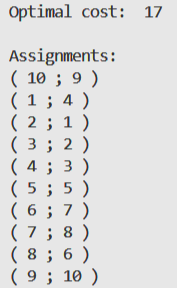
\includegraphics[]{венгерский метод.png}
\centering
\caption{Результат работы программы}
\end{figure}
